%\begin{center}

\vfill\null
\vspace{2cm}

\begin{figure}[H]
    \centering
    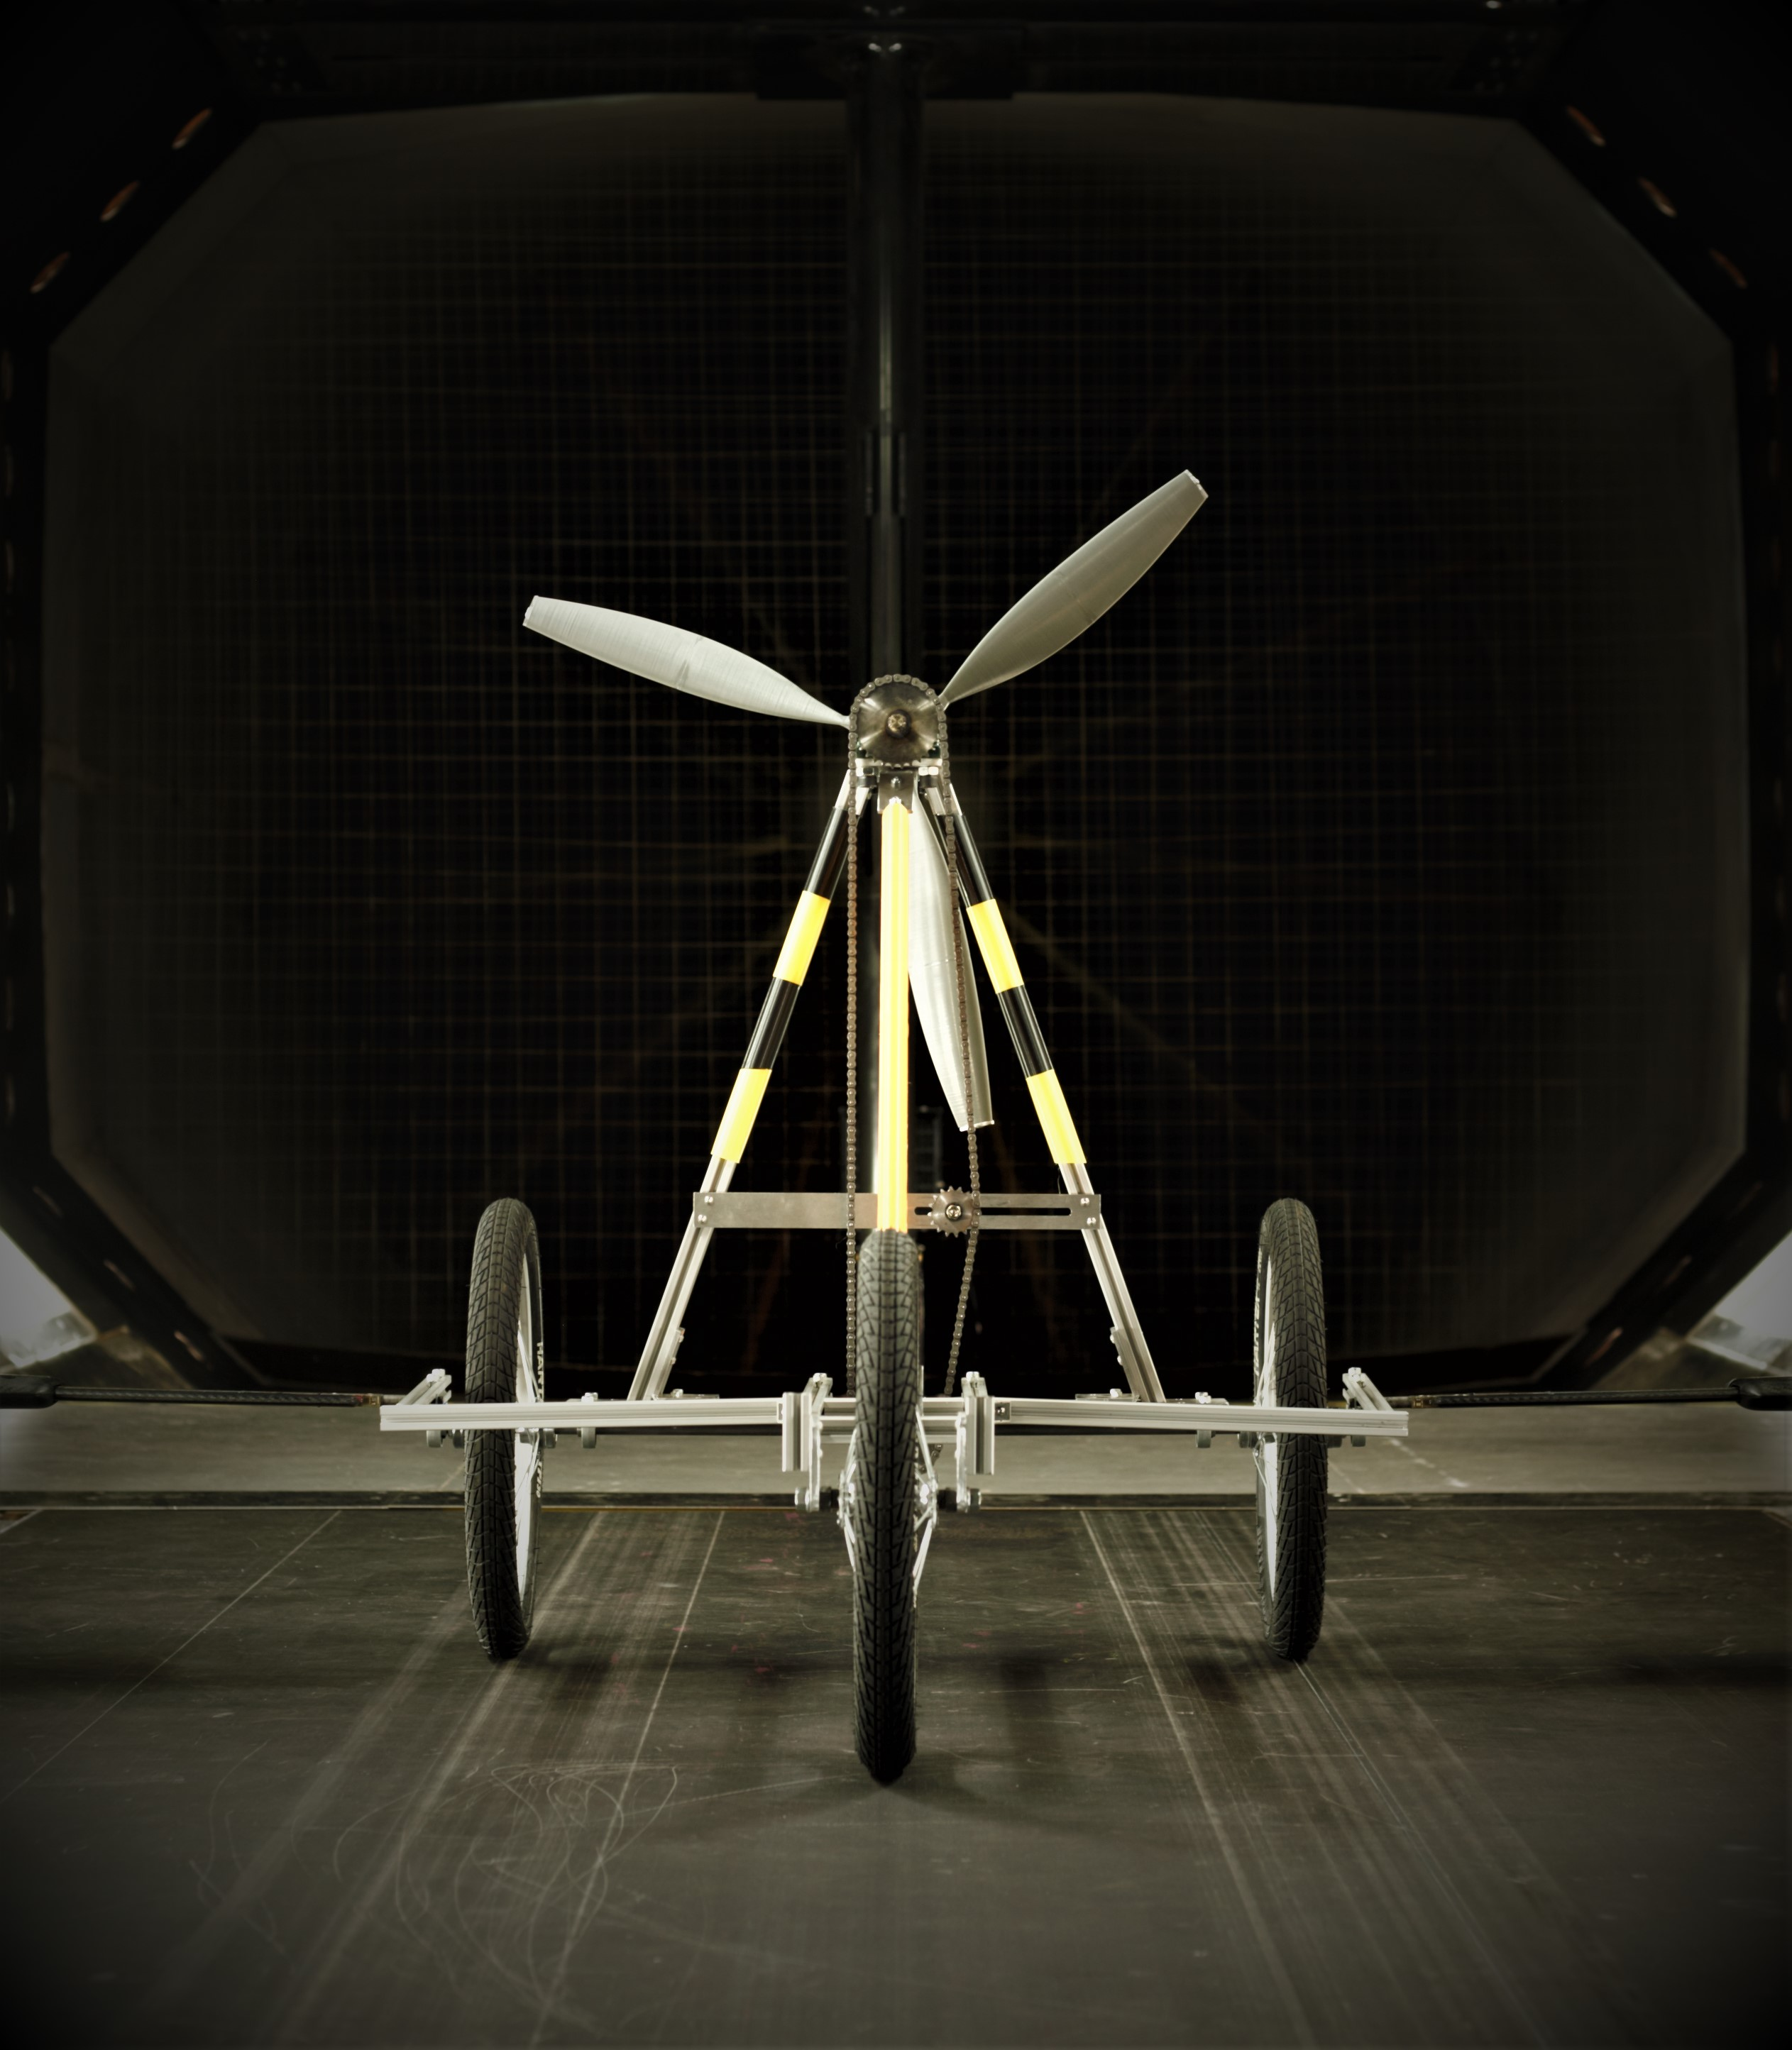
\includegraphics[width=\linewidth]{images/frontpage.jpg}
    \label{fig:frontpage}
\end{figure}

\vfill\null

\newpage


\noindent \textbf{Design Report}\\
\noindent {FEEG6013 Group Design Project}

\vspace{2cm}

\noindent {\Large \textbf{17}}

\vspace{0.3cm}

\noindent {\Large \textbf{Downwind Faster Than The Wind}}

\vspace{0.15cm}

\noindent Design, build and test a downwind-faster-than-the-wind vehicle
\vspace{1.5cm}

\noindent \subsubsection*{Project Summary:}

Downwind faster than the wind vehicles (DWFTTW) are wind-powered ground vehicles, capable of travelling dead-downwind, faster than the wind. A DWFTTW prototype featuring a 3D printed propeller with variable pitch capabilities and a modular chassis was designed, manufactured, and tested. All components featured on the vehicle were designed from scratch and a theoretical model, based on blade element theory, was created and used to optimise the design of the propeller and of the vehicle.

Experimental assessments of the prototype's characteristics were carried out in the R.J. Mitchell wind tunnel. The vehicle went through important structural changes to overcome flaws brought to light during the first session of wind tunnel experiments. It was then shown, during the second set of tests conducted, that the flaws had been overcome. The prototype was tested at operating speeds of up to $10 \mathrm{m/s}$ and the propeller at angular velocities of up to $470 \mathrm{RPM}$. 

Through analysis of experimental and numerical data, the overall performance of the vehicle was evaluated and an efficiency coefficient for the vehicle calculated. Conclusions were drawn on the key parameters implicated in the design of prototypes using this concept. Strategies for improving the vehicle performance were outlined.


\vspace{1.7cm}

\hrule

\vspace{1.3cm}

\noindent Group Members:
\begin{table}[H]
\begin{tabular}{lllll}
\textbf{ID Number} & \textbf{Name} & \hspace{1cm} & \textbf{ID Number} & \textbf{Name}       \\
30141508           & Iwan Tomos           &                   & 29323738          & Hadrien Develay\\
29370272           & Jean Fesquet         &                   & 28477235          & Alexander Hoad \\
29652987           & James Foggin         &                   & 29977916          & Simeon Young 
\end{tabular}

\end{table}							
\noindent Primary Supervisor: Dr Davide Lasagna \hspace{2cm} Co-Supervisor(s): Dr Ivo Peters
\vspace{12pt}
\newline \noindent Submitted on: 12/05/2022





\AddToShipoutPicture*{\put(950,750){
\includegraphics[width=6cm]{images/sotonLogo.png}}}





%\setcounter{page}{0}
\pagenumbering{gobble}
\newpage
\pagenumbering{arabic}















% \newcommand{\HRule}{\rule{\linewidth}{0.5mm}} % Defines a new command for the horizontal lines, change thickness here

% \center % Centre everything on the page

% \textsc{\LARGE University of Southampton}\\[7mm] % Name of your university/college
% 
\includegraphics[scale=.4]{images/crest.jpg}\\[0.5cm] % Include a department/university logo - this will require the graphicx package
% \textsc{\Large Aeronautics \& Astronautics}\\[0.15cm] % Major heading such as course name
% \textsc{\large Faculty of Engineering and Physical Sciences}\\[0.2cm] % Minor heading such as course title

% \HRule \\[4mm]
% { \huge \bfseries FEEG6013}\\[0.4cm]
% { \huge \bfseries GDP Group 17}\\[0.4cm]
% { \huge \bfseries Downwind-Faster-Than-The-Wind}\\[0.4cm]
% \HRule \\[2 cm]

% Group Members:\\
% \textbf{\emph{Hadrien DEVELAY -} 29323738}\\
% \textbf{\emph{Jean FESQUET -} 29370272}\\
% \textbf{\emph{James FOGGIN -} 29652987}\\
% \textbf{\emph{Alexander HOAD -} 28477235}\\
% \textbf{\emph{Iwan TOMOS -} 30141508}\\
% \textbf{\emph{Simeon YOUNG -} 29977916}\\[12mm]

% Primary Supervisor: \textbf{\emph{Davide LASAGNA}}\\
% Co-Supervisor: \textbf{\emph{Ivo PETERS}}\\[12 mm]


% %\vfill % Fill the rest of the page with whitespace


% Submitted on May 12\textsuperscript{th}, 2022\\[12mm] % Date, change the \today to a set date if you want to be precise

%\end{center}